% Options for packages loaded elsewhere
\PassOptionsToPackage{unicode}{hyperref}
\PassOptionsToPackage{hyphens}{url}
\PassOptionsToPackage{dvipsnames,svgnames,x11names}{xcolor}
%
\documentclass[
  letterpaper,
  DIV=11,
  numbers=noendperiod,
  oneside]{scrartcl}

\usepackage{amsmath,amssymb}
\usepackage{iftex}
\ifPDFTeX
  \usepackage[T1]{fontenc}
  \usepackage[utf8]{inputenc}
  \usepackage{textcomp} % provide euro and other symbols
\else % if luatex or xetex
  \usepackage{unicode-math}
  \defaultfontfeatures{Scale=MatchLowercase}
  \defaultfontfeatures[\rmfamily]{Ligatures=TeX,Scale=1}
\fi
\usepackage{lmodern}
\ifPDFTeX\else  
    % xetex/luatex font selection
\fi
% Use upquote if available, for straight quotes in verbatim environments
\IfFileExists{upquote.sty}{\usepackage{upquote}}{}
\IfFileExists{microtype.sty}{% use microtype if available
  \usepackage[]{microtype}
  \UseMicrotypeSet[protrusion]{basicmath} % disable protrusion for tt fonts
}{}
\makeatletter
\@ifundefined{KOMAClassName}{% if non-KOMA class
  \IfFileExists{parskip.sty}{%
    \usepackage{parskip}
  }{% else
    \setlength{\parindent}{0pt}
    \setlength{\parskip}{6pt plus 2pt minus 1pt}}
}{% if KOMA class
  \KOMAoptions{parskip=half}}
\makeatother
\usepackage{xcolor}
\usepackage[left=1in,marginparwidth=2.0666666666667in,textwidth=4.1333333333333in,marginparsep=0.3in]{geometry}
\setlength{\emergencystretch}{3em} % prevent overfull lines
\setcounter{secnumdepth}{-\maxdimen} % remove section numbering
% Make \paragraph and \subparagraph free-standing
\ifx\paragraph\undefined\else
  \let\oldparagraph\paragraph
  \renewcommand{\paragraph}[1]{\oldparagraph{#1}\mbox{}}
\fi
\ifx\subparagraph\undefined\else
  \let\oldsubparagraph\subparagraph
  \renewcommand{\subparagraph}[1]{\oldsubparagraph{#1}\mbox{}}
\fi

\usepackage{color}
\usepackage{fancyvrb}
\newcommand{\VerbBar}{|}
\newcommand{\VERB}{\Verb[commandchars=\\\{\}]}
\DefineVerbatimEnvironment{Highlighting}{Verbatim}{commandchars=\\\{\}}
% Add ',fontsize=\small' for more characters per line
\usepackage{framed}
\definecolor{shadecolor}{RGB}{241,243,245}
\newenvironment{Shaded}{\begin{snugshade}}{\end{snugshade}}
\newcommand{\AlertTok}[1]{\textcolor[rgb]{0.68,0.00,0.00}{#1}}
\newcommand{\AnnotationTok}[1]{\textcolor[rgb]{0.37,0.37,0.37}{#1}}
\newcommand{\AttributeTok}[1]{\textcolor[rgb]{0.40,0.45,0.13}{#1}}
\newcommand{\BaseNTok}[1]{\textcolor[rgb]{0.68,0.00,0.00}{#1}}
\newcommand{\BuiltInTok}[1]{\textcolor[rgb]{0.00,0.23,0.31}{#1}}
\newcommand{\CharTok}[1]{\textcolor[rgb]{0.13,0.47,0.30}{#1}}
\newcommand{\CommentTok}[1]{\textcolor[rgb]{0.37,0.37,0.37}{#1}}
\newcommand{\CommentVarTok}[1]{\textcolor[rgb]{0.37,0.37,0.37}{\textit{#1}}}
\newcommand{\ConstantTok}[1]{\textcolor[rgb]{0.56,0.35,0.01}{#1}}
\newcommand{\ControlFlowTok}[1]{\textcolor[rgb]{0.00,0.23,0.31}{\textbf{#1}}}
\newcommand{\DataTypeTok}[1]{\textcolor[rgb]{0.68,0.00,0.00}{#1}}
\newcommand{\DecValTok}[1]{\textcolor[rgb]{0.68,0.00,0.00}{#1}}
\newcommand{\DocumentationTok}[1]{\textcolor[rgb]{0.37,0.37,0.37}{\textit{#1}}}
\newcommand{\ErrorTok}[1]{\textcolor[rgb]{0.68,0.00,0.00}{#1}}
\newcommand{\ExtensionTok}[1]{\textcolor[rgb]{0.00,0.23,0.31}{#1}}
\newcommand{\FloatTok}[1]{\textcolor[rgb]{0.68,0.00,0.00}{#1}}
\newcommand{\FunctionTok}[1]{\textcolor[rgb]{0.28,0.35,0.67}{#1}}
\newcommand{\ImportTok}[1]{\textcolor[rgb]{0.00,0.46,0.62}{#1}}
\newcommand{\InformationTok}[1]{\textcolor[rgb]{0.37,0.37,0.37}{#1}}
\newcommand{\KeywordTok}[1]{\textcolor[rgb]{0.00,0.23,0.31}{\textbf{#1}}}
\newcommand{\NormalTok}[1]{\textcolor[rgb]{0.00,0.23,0.31}{#1}}
\newcommand{\OperatorTok}[1]{\textcolor[rgb]{0.37,0.37,0.37}{#1}}
\newcommand{\OtherTok}[1]{\textcolor[rgb]{0.00,0.23,0.31}{#1}}
\newcommand{\PreprocessorTok}[1]{\textcolor[rgb]{0.68,0.00,0.00}{#1}}
\newcommand{\RegionMarkerTok}[1]{\textcolor[rgb]{0.00,0.23,0.31}{#1}}
\newcommand{\SpecialCharTok}[1]{\textcolor[rgb]{0.37,0.37,0.37}{#1}}
\newcommand{\SpecialStringTok}[1]{\textcolor[rgb]{0.13,0.47,0.30}{#1}}
\newcommand{\StringTok}[1]{\textcolor[rgb]{0.13,0.47,0.30}{#1}}
\newcommand{\VariableTok}[1]{\textcolor[rgb]{0.07,0.07,0.07}{#1}}
\newcommand{\VerbatimStringTok}[1]{\textcolor[rgb]{0.13,0.47,0.30}{#1}}
\newcommand{\WarningTok}[1]{\textcolor[rgb]{0.37,0.37,0.37}{\textit{#1}}}

\providecommand{\tightlist}{%
  \setlength{\itemsep}{0pt}\setlength{\parskip}{0pt}}\usepackage{longtable,booktabs,array}
\usepackage{calc} % for calculating minipage widths
% Correct order of tables after \paragraph or \subparagraph
\usepackage{etoolbox}
\makeatletter
\patchcmd\longtable{\par}{\if@noskipsec\mbox{}\fi\par}{}{}
\makeatother
% Allow footnotes in longtable head/foot
\IfFileExists{footnotehyper.sty}{\usepackage{footnotehyper}}{\usepackage{footnote}}
\makesavenoteenv{longtable}
\usepackage{graphicx}
\makeatletter
\def\maxwidth{\ifdim\Gin@nat@width>\linewidth\linewidth\else\Gin@nat@width\fi}
\def\maxheight{\ifdim\Gin@nat@height>\textheight\textheight\else\Gin@nat@height\fi}
\makeatother
% Scale images if necessary, so that they will not overflow the page
% margins by default, and it is still possible to overwrite the defaults
% using explicit options in \includegraphics[width, height, ...]{}
\setkeys{Gin}{width=\maxwidth,height=\maxheight,keepaspectratio}
% Set default figure placement to htbp
\makeatletter
\def\fps@figure{htbp}
\makeatother

\KOMAoption{captions}{tableheading}
\makeatletter
\@ifpackageloaded{tcolorbox}{}{\usepackage[skins,breakable]{tcolorbox}}
\@ifpackageloaded{fontawesome5}{}{\usepackage{fontawesome5}}
\definecolor{quarto-callout-color}{HTML}{909090}
\definecolor{quarto-callout-note-color}{HTML}{0758E5}
\definecolor{quarto-callout-important-color}{HTML}{CC1914}
\definecolor{quarto-callout-warning-color}{HTML}{EB9113}
\definecolor{quarto-callout-tip-color}{HTML}{00A047}
\definecolor{quarto-callout-caution-color}{HTML}{FC5300}
\definecolor{quarto-callout-color-frame}{HTML}{acacac}
\definecolor{quarto-callout-note-color-frame}{HTML}{4582ec}
\definecolor{quarto-callout-important-color-frame}{HTML}{d9534f}
\definecolor{quarto-callout-warning-color-frame}{HTML}{f0ad4e}
\definecolor{quarto-callout-tip-color-frame}{HTML}{02b875}
\definecolor{quarto-callout-caution-color-frame}{HTML}{fd7e14}
\makeatother
\makeatletter
\@ifpackageloaded{caption}{}{\usepackage{caption}}
\AtBeginDocument{%
\ifdefined\contentsname
  \renewcommand*\contentsname{Table of contents}
\else
  \newcommand\contentsname{Table of contents}
\fi
\ifdefined\listfigurename
  \renewcommand*\listfigurename{List of Figures}
\else
  \newcommand\listfigurename{List of Figures}
\fi
\ifdefined\listtablename
  \renewcommand*\listtablename{List of Tables}
\else
  \newcommand\listtablename{List of Tables}
\fi
\ifdefined\figurename
  \renewcommand*\figurename{Figure}
\else
  \newcommand\figurename{Figure}
\fi
\ifdefined\tablename
  \renewcommand*\tablename{Table}
\else
  \newcommand\tablename{Table}
\fi
}
\@ifpackageloaded{float}{}{\usepackage{float}}
\floatstyle{ruled}
\@ifundefined{c@chapter}{\newfloat{codelisting}{h}{lop}}{\newfloat{codelisting}{h}{lop}[chapter]}
\floatname{codelisting}{Listing}
\newcommand*\listoflistings{\listof{codelisting}{List of Listings}}
\makeatother
\makeatletter
\makeatother
\makeatletter
\@ifpackageloaded{caption}{}{\usepackage{caption}}
\@ifpackageloaded{subcaption}{}{\usepackage{subcaption}}
\makeatother
\makeatletter
\@ifpackageloaded{sidenotes}{}{\usepackage{sidenotes}}
\@ifpackageloaded{marginnote}{}{\usepackage{marginnote}}
\makeatother
\makeatletter
\@ifpackageloaded{fontawesome5}{}{\usepackage{fontawesome5}}
\makeatother
\ifLuaTeX
  \usepackage{selnolig}  % disable illegal ligatures
\fi
\usepackage{bookmark}

\IfFileExists{xurl.sty}{\usepackage{xurl}}{} % add URL line breaks if available
\urlstyle{same} % disable monospaced font for URLs
\hypersetup{
  pdftitle={Repo Security},
  pdfauthor={Frank Aragona; Kathleen Conery},
  colorlinks=true,
  linkcolor={blue},
  filecolor={Maroon},
  citecolor={Blue},
  urlcolor={Blue},
  pdfcreator={LaTeX via pandoc}}

\title{Repo Security}
\author{Frank Aragona \and Kathleen Conery}
\date{2023-04-09}

\begin{document}
\maketitle

\faIcon{unlock} \textbf{Objectives}

\begin{itemize}
\tightlist
\item
  Prevent sensitive information leaks to Github
\item
  Set up guardrails, \texttt{.gitignore}, hooks
\item
  Scrub private repos before they go public
\end{itemize}

If sensitive information is leaked and commited to the remote repo, then
they will stay in the git history (and will require a lot of effort to
remove them from the history). The following cannot be included in any
repo \textbf{or any local commit!}:

\begin{longtable}[]{@{}
  >{\raggedright\arraybackslash}p{(\columnwidth - 2\tabcolsep) * \real{0.3750}}
  >{\raggedright\arraybackslash}p{(\columnwidth - 2\tabcolsep) * \real{0.5833}}@{}}
\toprule\noalign{}
\begin{minipage}[b]{\linewidth}\raggedright
Type
\end{minipage} & \begin{minipage}[b]{\linewidth}\raggedright
Examples
\end{minipage} \\
\midrule\noalign{}
\endhead
\bottomrule\noalign{}
\endlastfoot
File Paths & \begin{minipage}[t]{\linewidth}\raggedright
\begin{itemize}
\tightlist
\item
  Network drives
\item
  Shared internal drives
\end{itemize}
\end{minipage} \\
Server Names & \begin{minipage}[t]{\linewidth}\raggedright
\begin{itemize}
\tightlist
\item
  ODBC Connections
\end{itemize}
\end{minipage} \\
Credentials & \begin{minipage}[t]{\linewidth}\raggedright
\begin{itemize}
\tightlist
\item
  SSH Keys
\item
  Tokens (REDCap, Azure, Github, etc)
\item
  Usernames
\item
  Passwords
\item
  Blob/bucket keys
\end{itemize}
\end{minipage} \\
Identifiable Information & \begin{minipage}[t]{\linewidth}\raggedright
\begin{itemize}
\tightlist
\item
  Addresses
\item
  Names
\item
  Any PHI
\end{itemize}
\end{minipage} \\
\end{longtable}

\subsection*{Prevent Credential Leaks with Env
Variables}\label{prevent-credential-leaks-with-env-variables}
\addcontentsline{toc}{subsection}{Prevent Credential Leaks with Env
Variables}

There are a number of ways to do this. We typically use a yaml file that
can be filled out with personal credentials locally. The file will not
be committed to the remote repo

\subsubsection{Create a private credentials
file}\label{create-a-private-credentials-file}

The scripts use a \texttt{.yml} file that contains a list of API tokens,
server names, and usernames/passwords specific to each individual user.
There are two \texttt{.yml} files. One is a template (containing no
actual passwords..) that exists in the repo and serves as a template so
every individual user can keep up to date with new credential additions.
The other is the individual \texttt{creds.yml} that is in the repo's
\texttt{.gitignore}. This file will never exist in the repo and only
exist locally (in the user's C drive).

\subsubsection{\texorpdfstring{\texttt{creds.yml}
details}{creds.yml details}}\label{creds.yml-details}

The \texttt{.yml} file can work with multiple programming languages
including R and Python. They are read in the same way and can be easily
adjusted when adding new passwords or using them as configuration files.

They look like this:

\begin{codelisting}

\caption{\texttt{local-credentials.yml}}

\begin{Shaded}
\begin{Highlighting}[]
\CommentTok{\# Default is needed to distinguish values.}
\CommentTok{\# Leave a blank line (NO SPACES) as the last line in this file or things will break}
\CommentTok{\# Quotes aren\textquotesingle{}t necessary, but can be used.}
\FunctionTok{default}\KeywordTok{:}\AttributeTok{ }
\AttributeTok{  }\FunctionTok{conn\_list\_wdrs}\KeywordTok{:}
\AttributeTok{    }\FunctionTok{Driver}\KeywordTok{:}\AttributeTok{ }\StringTok{"SQL Server Native Client 11.0"}
\AttributeTok{    }\FunctionTok{Server}\KeywordTok{:}\AttributeTok{ }
\AttributeTok{    }\FunctionTok{Database}\KeywordTok{:}\AttributeTok{ }
\AttributeTok{    }\FunctionTok{Trusted\_connection}\KeywordTok{:}\AttributeTok{ }
\AttributeTok{    }\FunctionTok{ApplicationIntent}\KeywordTok{:}\AttributeTok{ }
\AttributeTok{    }
\AttributeTok{  }\FunctionTok{fulgent}\KeywordTok{:}
\AttributeTok{    }\FunctionTok{username}\KeywordTok{:}\AttributeTok{ \textless{}USERNAME\textgreater{}}
\AttributeTok{    }\FunctionTok{password}\KeywordTok{:}\AttributeTok{ \textless{}PASSWORD\textgreater{}}
\end{Highlighting}
\end{Shaded}

\end{codelisting}

You can have different variables assigned to unique lists, which allows
for easy configuration. For example, the list starting with
\texttt{default} has variables \texttt{conn\_list\_wdrs} and
\texttt{fulgent}. You can have a different list of variables within the
same file like this:

\begin{codelisting}

\caption{\texttt{local-credentials.yml}}

\begin{Shaded}
\begin{Highlighting}[]
\CommentTok{\# Default is needed to distinguish values.}
\CommentTok{\# Leave a blank line (NO SPACES) as the last line in this file or things will break}
\CommentTok{\# Quotes aren\textquotesingle{}t necessary, but can be used.}
\FunctionTok{default}\KeywordTok{:}\AttributeTok{ }
\AttributeTok{  }\FunctionTok{conn\_list\_wdrs}\KeywordTok{:}
\AttributeTok{    }\FunctionTok{Driver}\KeywordTok{:}\AttributeTok{ }\StringTok{"SQL Server Native Client 11.0"}
\AttributeTok{    }\FunctionTok{Server}\KeywordTok{:}\AttributeTok{ }
\AttributeTok{    }\FunctionTok{Database}\KeywordTok{:}\AttributeTok{ }
\AttributeTok{    }\FunctionTok{Trusted\_connection}\KeywordTok{:}\AttributeTok{ }
\AttributeTok{    }\FunctionTok{ApplicationIntent}\KeywordTok{:}\AttributeTok{ }
\AttributeTok{    }
\AttributeTok{  }\FunctionTok{fulgent}\KeywordTok{:}
\AttributeTok{    }\FunctionTok{username}\KeywordTok{:}\AttributeTok{ \textless{}USERNAME\textgreater{}}
\AttributeTok{    }\FunctionTok{password}\KeywordTok{:}\AttributeTok{ \textless{}PASSWORD\textgreater{}}

\FunctionTok{test}\KeywordTok{:}
\AttributeTok{  }\FunctionTok{conn\_list\_wdrs}\KeywordTok{:}
\AttributeTok{    }\FunctionTok{Driver}\KeywordTok{:}\AttributeTok{ }\StringTok{"SQL Server Native Client 11.0"}
\AttributeTok{    }\FunctionTok{Server}\KeywordTok{:}\AttributeTok{ }
\AttributeTok{    }\FunctionTok{Database}\KeywordTok{:}\AttributeTok{ }
\AttributeTok{    }\FunctionTok{Trusted\_connection}\KeywordTok{:}\AttributeTok{ }
\AttributeTok{    }\FunctionTok{ApplicationIntent}\KeywordTok{:}\AttributeTok{ }
\end{Highlighting}
\end{Shaded}

\end{codelisting}

Now there is a \texttt{test} list with its own variables. This lets us
switch a set of variables within our scripts. \texttt{default} applies
to the main credentials where \texttt{test} can distinguish which
variables should be test or dev scripts specific. Notice below that you
can now call the credentials from a \texttt{.yml} file into an R or
Python script and the actual credentials will never exist in the code
pushed to the repo.

\begin{codelisting}

\caption{\texttt{script-in-repo.R}}

\begin{Shaded}
\begin{Highlighting}[]
\CommentTok{\# this script is in the repo, but credentials are hidden}
\FunctionTok{library}\NormalTok{(yaml)}

\CommentTok{\# read in the local credentials yaml file}
\NormalTok{creds }\OtherTok{\textless{}{-}}\NormalTok{ yaml}\SpecialCharTok{::}\FunctionTok{read\_yaml}\NormalTok{(}\StringTok{"path/to/local{-}credentials.yml"}\NormalTok{)}

\CommentTok{\# pull in the credentials}
\NormalTok{server\_name }\OtherTok{\textless{}{-}}\NormalTok{ creds}\SpecialCharTok{$}\NormalTok{default}\SpecialCharTok{$}\NormalTok{conn\_list\_wdrs}\SpecialCharTok{$}\NormalTok{server}
\end{Highlighting}
\end{Shaded}

\end{codelisting}

\newpage{}

:::: \{.content-visible unless-format=``pdf''\} \#\#\# \{.unnumbered\}

\begin{figure*}

We can even get more specific and add an \texttt{if-else} statement to
specify which credential we want to select. This can be helpful if we
have a CI/CD pipeline and have a script automatically run on a task
scheduler or cron job. We can call the credentials we want in the
command line and have the command line code run in my task scheduler.
That way we can use multiple different versions of the same script and
have all of it be automated.

For example, the middle panel uses the \texttt{commandArgs()} to pull
any arguments passed to the script in a shell/command line script. In
the right panel, the shell script has \texttt{production} and
\texttt{test} as second arguments. These are passed to the R script as
\texttt{arg{[}2{]}}. Now we can use \texttt{arg{[}2{]}} in the if-else
statement to conditionally select credentials and do it automatically.

\begin{codelisting}

\caption{\texttt{script-in-repo.R}}

\begin{Shaded}
\begin{Highlighting}[]
\NormalTok{args }\OtherTok{\textless{}{-}} \FunctionTok{commandArgs}\NormalTok{(}\ConstantTok{TRUE}\NormalTok{)}

\CommentTok{\# this script is in the repo, but credentials are hidden}
\FunctionTok{library}\NormalTok{(yaml)}

\CommentTok{\# read in the local credentials yaml file}
\NormalTok{creds }\OtherTok{\textless{}{-}}\NormalTok{ yaml}\SpecialCharTok{::}\FunctionTok{read\_yaml}\NormalTok{(}\StringTok{"path/to/local{-}credentials.yml"}\NormalTok{)}

\CommentTok{\# pull in the credentials}
\ControlFlowTok{if}\NormalTok{(args[}\DecValTok{2}\NormalTok{] }\SpecialCharTok{==} \StringTok{"production"}\NormalTok{)\{}
\NormalTok{  server\_name }\OtherTok{\textless{}{-}}\NormalTok{ creds}\SpecialCharTok{$}\NormalTok{default}\SpecialCharTok{$}\NormalTok{conn\_list\_wdrs}\SpecialCharTok{$}\NormalTok{server}
\NormalTok{\} }\ControlFlowTok{else} \ControlFlowTok{if}\NormalTok{(args[}\DecValTok{2}\NormalTok{] }\SpecialCharTok{==} \StringTok{"test"}\NormalTok{)\{}
\NormalTok{  server\_name }\OtherTok{\textless{}{-}}\NormalTok{ creds}\SpecialCharTok{$}\NormalTok{test}\SpecialCharTok{$}\NormalTok{conn\_list\_wdrs}\SpecialCharTok{$}\NormalTok{server}
\NormalTok{\}}
\end{Highlighting}
\end{Shaded}

\end{codelisting}

\begin{codelisting}

\caption{\texttt{shell-trigger-script.sh}}

\begin{Shaded}
\begin{Highlighting}[]
\CommentTok{\# Run the production code}
\ExtensionTok{$}\NormalTok{ Rscript }\AttributeTok{{-}e} \StringTok{"source(\textquotesingle{}path/script\_in\_repo.R\textquotesingle{});"}\NormalTok{ production}

\CommentTok{\# Run the test/dev code}
\ExtensionTok{$}\NormalTok{ Rscript }\AttributeTok{{-}e} \StringTok{"source(\textquotesingle{}path/script\_in\_repo.R\textquotesingle{});"}\NormalTok{ test }
\end{Highlighting}
\end{Shaded}

\end{codelisting}

\end{figure*}%

\newpage{}

We can even get more specific and add an \texttt{if-else} statement to
specify which credential we want to select. This can be helpful if we
have a CI/CD pipeline and have a script automatically run on a task
scheduler or cron job. We can call the credentials we want in the
command line and have the command line code run in my task scheduler.
That way we can use multiple different versions of the same script and
have all of it be automated.

For example, the middle panel uses the \texttt{commandArgs()} to pull
any arguments passed to the script in a shell/command line script. In
the right panel, the shell script has \texttt{production} and
\texttt{test} as second arguments. These are passed to the R script as
\texttt{arg{[}2{]}}. Now we can use \texttt{arg{[}2{]}} in the if-else
statement to conditionally select credentials and do it automatically.

\begin{codelisting}

\caption{\texttt{script-in-repo.R}}

\begin{Shaded}
\begin{Highlighting}[]
\NormalTok{args }\OtherTok{\textless{}{-}} \FunctionTok{commandArgs}\NormalTok{(}\ConstantTok{TRUE}\NormalTok{)}

\CommentTok{\# this script is in the repo, but credentials are hidden}
\FunctionTok{library}\NormalTok{(yaml)}

\CommentTok{\# read in the local credentials yaml file}
\NormalTok{creds }\OtherTok{\textless{}{-}}\NormalTok{ yaml}\SpecialCharTok{::}\FunctionTok{read\_yaml}\NormalTok{(}\StringTok{"path/to/local{-}credentials.yml"}\NormalTok{)}

\CommentTok{\# pull in the credentials}
\ControlFlowTok{if}\NormalTok{(args[}\DecValTok{2}\NormalTok{] }\SpecialCharTok{==} \StringTok{"production"}\NormalTok{)\{}
\NormalTok{  server\_name }\OtherTok{\textless{}{-}}\NormalTok{ creds}\SpecialCharTok{$}\NormalTok{default}\SpecialCharTok{$}\NormalTok{conn\_list\_wdrs}\SpecialCharTok{$}\NormalTok{server}
\NormalTok{\} }\ControlFlowTok{else} \ControlFlowTok{if}\NormalTok{(args[}\DecValTok{2}\NormalTok{] }\SpecialCharTok{==} \StringTok{"test"}\NormalTok{)\{}
\NormalTok{  server\_name }\OtherTok{\textless{}{-}}\NormalTok{ creds}\SpecialCharTok{$}\NormalTok{test}\SpecialCharTok{$}\NormalTok{conn\_list\_wdrs}\SpecialCharTok{$}\NormalTok{server}
\NormalTok{\}}
\end{Highlighting}
\end{Shaded}

\end{codelisting}

\begin{codelisting}

\caption{\texttt{shell-trigger-script.sh}}

\begin{Shaded}
\begin{Highlighting}[]
\CommentTok{\# Run the production code}
\ExtensionTok{$}\NormalTok{ Rscript }\AttributeTok{{-}e} \StringTok{"source(\textquotesingle{}path/script\_in\_repo.R\textquotesingle{});"}\NormalTok{ production}

\CommentTok{\# Run the test/dev code}
\ExtensionTok{$}\NormalTok{ Rscript }\AttributeTok{{-}e} \StringTok{"source(\textquotesingle{}path/script\_in\_repo.R\textquotesingle{});"}\NormalTok{ test }
\end{Highlighting}
\end{Shaded}

\end{codelisting}

\newpage{}

\subsubsection{Safe Guards - Prevent Accidental
Leaks!}\label{safe-guards---prevent-accidental-leaks}

Once you have the credentials.yml template in your repo, make sure that
nobody on your team (or anyone with write access..) is able to
accidentally push changes to the template. We don't want someone's
passwords or API tokens to exist in GitHub.

\href{https://stackoverflow.com/a/39776107}{This link shows how to skip
any changes made to the specific file}. If someone makes local changes
to the template, the changes will not show in their commit. It is a safe
guard.

\paragraph{For all individual users, run this
code:}\label{for-all-individual-users-run-this-code}

\begin{Shaded}
\begin{Highlighting}[]
\FunctionTok{git}\NormalTok{ update{-}index }\AttributeTok{{-}{-}skip{-}worktree}\NormalTok{ creds\_TEMPLATE.yml}
\end{Highlighting}
\end{Shaded}

This will tell your local git to ignore any changes made to
\texttt{creds\_TEMPLATE.yml}, but also allow it to exist in the repo
(since \texttt{.gitignore} will prevent it from being in the repo)

\paragraph{If you need to update the template file run
this:}\label{if-you-need-to-update-the-template-file-run-this}

\begin{Shaded}
\begin{Highlighting}[]
\FunctionTok{git}\NormalTok{ update{-}index }\AttributeTok{{-}{-}no{-}skip{-}worktree}\NormalTok{ creds\_TEMPLATE.yml}
\end{Highlighting}
\end{Shaded}

This will allow changes to the template. \textbf{So when you need to
update the template, use this code}

And to get a list of files that are ``skipped'', use this code:

\begin{Shaded}
\begin{Highlighting}[]
\FunctionTok{git}\NormalTok{ ls{-}files }\AttributeTok{{-}v}\NormalTok{ . }\KeywordTok{|} \FunctionTok{grep}\NormalTok{ \^{}S}
\end{Highlighting}
\end{Shaded}

\newpage{}

\section{Security Guardrails}\label{security-guardrails}

Using a \texttt{.gitignore} file for environmental variables/credentials
is an excellent guardrail and promotes good coding habits, but we may
also want additional guardrails such as hooks.

Hooks are processes that run in the background and can prevent code from
being pushed if there is a security flaw. There are two hooks we could
use for security; pre-commit hooks and pre-receive hooks

\subsection{Pre-commit Hooks}\label{pre-commit-hooks}

Pre-commit hooks run a process locally when the user attempts to commit
code to a git branch. Hooks have many uses. Here we can use them as a
security guardrail to prevent accidental credential leaks in committed
code.

\begin{enumerate}
\def\labelenumi{\arabic{enumi}.}
\item
  Clone or download the AWS Git Secrets repo from
  \href{https://github.com/awslabs/git-secrets/blob/master/install.ps1}{awslabs
  GitHub}

  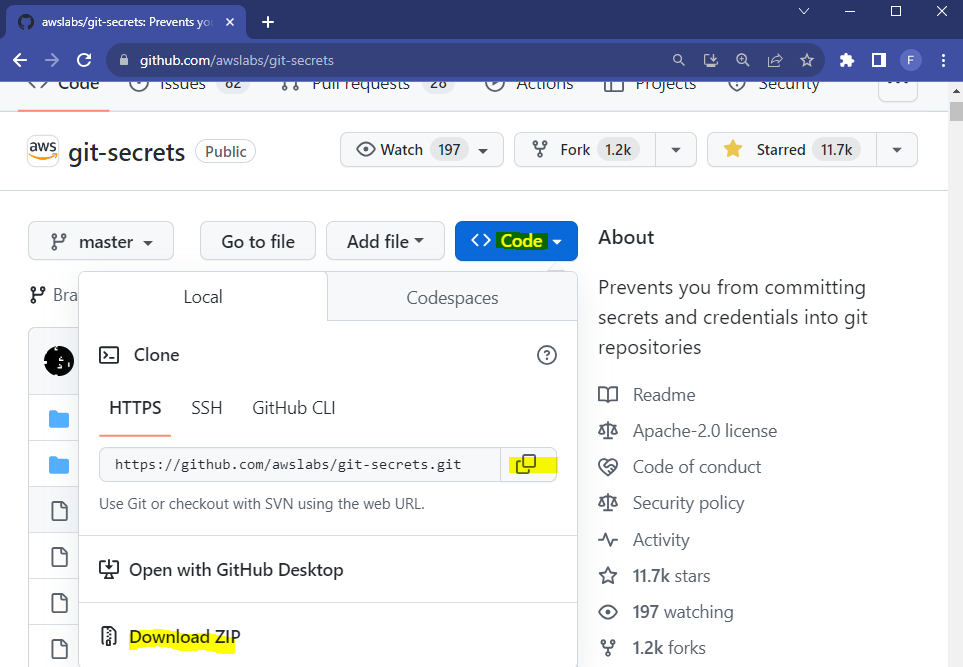
\includegraphics{images/gh_secrets.PNG}
\item
  Extract zip
\item
  Open folder and right click install.ps1

  \begin{enumerate}
  \def\labelenumii{\alph{enumii}.}
  \tightlist
  \item
    Run in Power Shell
  \item
    Type Y to give permission
  \end{enumerate}
\item
  CD to a directory where you have the git repository you want to
  upload, either in PowerShell or R studio terminal \faIcon{terminal}

  \begin{codelisting}

  \caption{\texttt{PowerShell}}

\begin{Shaded}
\begin{Highlighting}[]
\ExtensionTok{PS} \OperatorTok{\textgreater{}}\NormalTok{ cd path/to/repo/root}
\end{Highlighting}
\end{Shaded}

  \end{codelisting}
\item
  Run git secrets --install

  \begin{codelisting}

  \caption{\texttt{PowerShell}}

\begin{Shaded}
\begin{Highlighting}[]
\FunctionTok{git}\NormalTok{ secrets }\AttributeTok{{-}{-}install}
\end{Highlighting}
\end{Shaded}

  \end{codelisting}
\item
  Make or copy the regex file called \texttt{secrets\_key} containing
  the secret patterns into your folder. -- make text file -- discuss
  with team what all we want to make illegal.
\item
  Make sure the file \texttt{secrets\_key} is in your
  \texttt{.gitignore}. We can't push that to the remote repo.
\item
  Run \texttt{git\ secrets\ -\/-add-provider\ -\/-\ cat\ ./secrets\_key}

  \begin{codelisting}

  \caption{\texttt{PowerShell}}

\begin{Shaded}
\begin{Highlighting}[]
\FunctionTok{git}\NormalTok{ secrets }\AttributeTok{{-}{-}add{-}provider} \AttributeTok{{-}{-}}\NormalTok{ cat ./secrets\_key}
\end{Highlighting}
\end{Shaded}

  \end{codelisting}

  You can also add prohibited patterns like this

  \begin{codelisting}

  \caption{\texttt{PowerShell}}

\begin{Shaded}
\begin{Highlighting}[]
\CommentTok{\# add a pattern}
\FunctionTok{git}\NormalTok{ secrets }\AttributeTok{{-}{-}add} \StringTok{\textquotesingle{}[A{-}Z0{-}9]\{20\}\textquotesingle{}}

\CommentTok{\# add a literal string, the + is escaped}
\FunctionTok{git}\NormalTok{ secrets }\AttributeTok{{-}{-}add} \AttributeTok{{-}{-}literal} \StringTok{\textquotesingle{}foo+bar\textquotesingle{}}

\CommentTok{\# add an allowed pattern}
\FunctionTok{git}\NormalTok{ secrets }\AttributeTok{{-}{-}add} \AttributeTok{{-}a} \StringTok{\textquotesingle{}allowed pattern\textquotesingle{}}
\end{Highlighting}
\end{Shaded}

  \end{codelisting}
\item
  Test Git history by running

  \begin{codelisting}

  \caption{\texttt{PowerShell}}

\begin{Shaded}
\begin{Highlighting}[]
\FunctionTok{git}\NormalTok{ secrets }\AttributeTok{{-}{-}scan{-}history}
\end{Highlighting}
\end{Shaded}

  \end{codelisting}
\item
  If something gets flagged and you don't care about your history
  anymore: Delete .git folder and reinitialize repository

  I would take caution about this point. There might be better ways to
  clean your git history if you don't want to get rid of everything.
\item
  Test on one of my projects to see if rebasing is a sustainable option
\item
  Make repo public
\item
  Will automatically scan on every commit and won't let it commit unless
  it's clean - Create a few files to show it working
\end{enumerate}

\begin{tcolorbox}[enhanced jigsaw, opacitybacktitle=0.6, bottomrule=.15mm, arc=.35mm, colframe=quarto-callout-note-color-frame, breakable, toptitle=1mm, bottomtitle=1mm, left=2mm, coltitle=black, opacityback=0, titlerule=0mm, toprule=.15mm, title=\textcolor{quarto-callout-note-color}{\faInfo}\hspace{0.5em}{Note}, colbacktitle=quarto-callout-note-color!10!white, rightrule=.15mm, leftrule=.75mm, colback=white]

We can't use the ``Non capture group'' feature of regex. Meaning we
can't use patterns like this in our regex: (?:abc) -- see
https://regexr.com IMPORTANT: Tab separate your regex expressions.
Making new lines caused a bit of chaos and took really long to figure
out. (you can use multiple tabs to separate them more visually)

\end{tcolorbox}

\faIcon{unlock} \textbf{NOTE!!}

\begin{itemize}
\tightlist
\item
  The REGEX strings used in the \texttt{secrets\_key} file may be
  decieving
\item
  Make sure to test that the regex flags what you want it to
\item
  \texttt{git\ secrets\ -\/-scan-history} may take a very long time to
  run
\end{itemize}

\begin{enumerate}
\def\labelenumi{\arabic{enumi}.}
\item
  Check that the \texttt{secrets\_key} regex is working by running the
  process on a repo that you know has secrets in it. For example, in a
  different folder, run all the pre-commit hook steps above and add a
  known ``bad'' string into the regex. For example, in the regex put
  \texttt{bad\_string} and in a file in that folder put
  \texttt{bad\_string}. When you scan it should get flagged.
\item
  If secret scanning is taking too long, you might want to check certain
  files first. I've found that HTML files take a \emph{very} long time
  to scan for secrets. If you're using linux or macOS you should be able
  to scan certain files via grob like this
  \texttt{git\ secrets\ -\/-scan\ path/to/files*}. If you're using
  windows it probably won't work. In that case, if you only want certain
  file extentsions to be scanned, use this function in powershell below.
  Download the file here:
\end{enumerate}

\begin{codelisting}

\caption{\texttt{secret-scanner9000.ps1}}

\begin{Shaded}
\begin{Highlighting}[]
\CommentTok{\# Example Usage}
\CommentTok{\# write this in the powershell terminal, adjust for the file type(s) you want to scan {-} can be multiple types: $fileExtensions = @(".R", ".py")}
\CommentTok{\# then execute this in the terminal: ScanFiles {-}FileExtensions $fileExtensions}

\CommentTok{\# It will give you an output of any secrets that are contained in those files}

\ExtensionTok{Function}\NormalTok{ ScanFiles\{}
  \ExtensionTok{param} \ErrorTok{(}
      \ExtensionTok{[string]}\VariableTok{$filePath}\NormalTok{ = }\ErrorTok{(}\ExtensionTok{Get{-}Location}\KeywordTok{)}\ExtensionTok{.Path,}
      \ExtensionTok{[string[]]}\VariableTok{$fileExtensions}
\KeywordTok{)} 
  \ExtensionTok{Get{-}ChildItem} \VariableTok{$filePath} \AttributeTok{{-}recurse} \KeywordTok{|} \ExtensionTok{Where{-}Object}\NormalTok{ \{}\VariableTok{$\_}\NormalTok{.extension }\AttributeTok{{-}in} \VariableTok{$fileExtensions}\NormalTok{\} }\KeywordTok{|} 
  \ExtensionTok{Foreach{-}Object}\NormalTok{ \{}

      \FunctionTok{git}\NormalTok{ secrets }\AttributeTok{{-}{-}scan} \VariableTok{$\_}\NormalTok{.FullName }\KeywordTok{|} \ExtensionTok{Out{-}File} \VariableTok{$logFile} \AttributeTok{{-}Append}

  \ErrorTok{\}}
\ErrorTok{\}}
\end{Highlighting}
\end{Shaded}

\end{codelisting}

Now, you can scan your secrets by copying and pasting the code into a
powershell terminal like this:

\begin{codelisting}

\caption{\texttt{PowerShell}}

\begin{Shaded}
\begin{Highlighting}[]
\VariableTok{$fileExtensions}\NormalTok{ = }\PreprocessorTok{@(}\StringTok{".R"}\NormalTok{,}\StringTok{".py"}\NormalTok{,}\StringTok{".Rmd"}\NormalTok{,}\StringTok{".qmd"}\PreprocessorTok{)}
\ExtensionTok{ScanFiles} \AttributeTok{{-}FileExtensions} \VariableTok{$fileExtensions}
\end{Highlighting}
\end{Shaded}

\end{codelisting}

\newpage{}

\subsection{Pre-Recieve Hooks}\label{pre-recieve-hooks}

These are still being investigated. They are remote hooks (not local
like pre-commit hooks) that can be deployed throughout the Github
organization. They can block certain commits from ever being pushed to
the remote repo. They may make things unnecessarily complicated

\subsection{Pushing Private Code to Public
Repos}\label{pushing-private-code-to-public-repos}

We may wish to take private codes and push them to a public repo. We
need to make sure that the public code doesn't not contain sensitive or
forbidden data/code, so cleaning up the private repo is important before
pushing.

There are a few ways to do this, but the easiest way is to copy the
clean private code to the public repo, that is, copy all the files you
want to add publicly but \textbf{do not copy the \texttt{.git}} folder.
If the private repo has a dirty git history we will not want that
history in the public repo because the sensitive data will then be
publicly available.

\begin{figure*}

\begin{minipage}{0.50\linewidth}
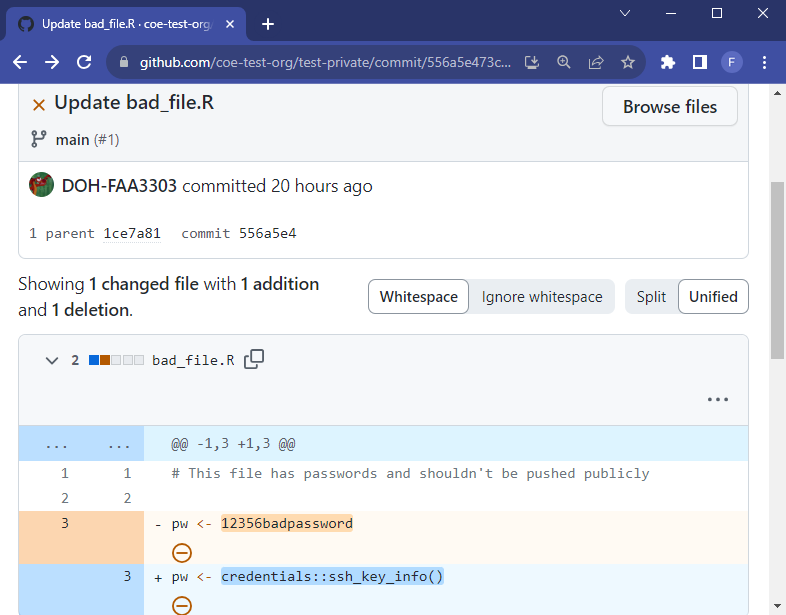
\includegraphics{images/private_repo3.PNG}\end{minipage}%
%
\begin{minipage}{0.50\linewidth}
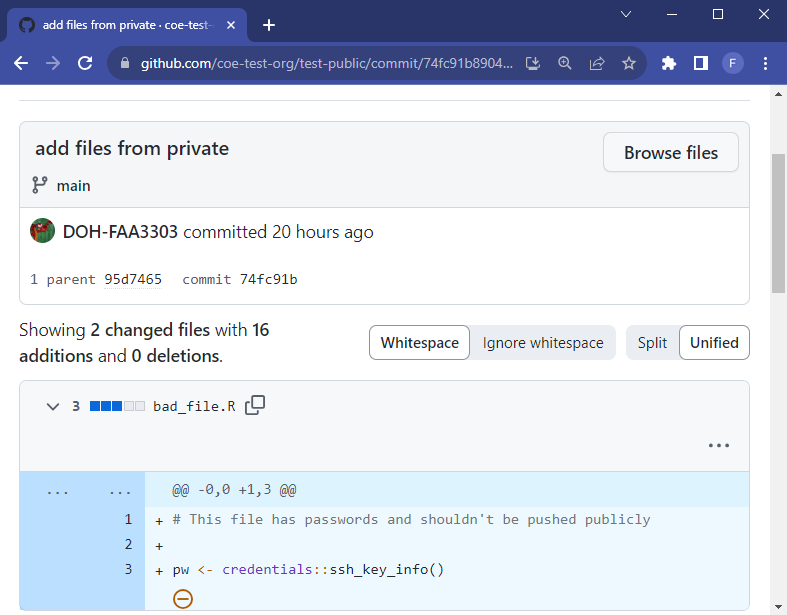
\includegraphics{images/public_repo3.PNG}\end{minipage}%

\end{figure*}%

\faIcon{exclamation} The private repository on the left still contains
sensitive information in the git history. The public repository on the
right has a clean git history because we copied only the current clean
files from the private repo and did not attach its git history (which
lives in the hidden \texttt{.git} folder)

\section{Code Reviewers/Github Operations
Team}\label{code-reviewersgithub-operations-team}

With the guardrails above in place there should be few chances that
credentials get pushed to a repo. However accidents may still happen. We
want to make sure that anyone who opens up a repo in the Github
organization adheres to the rules, has the proper credential/coding
set-up, and installs their local pre-commit hooks properly.

It may be useful to have a team within the organization that helps with
repo set-up. The team would help avoid a scenario where a person opens
up a repo without reading this documentation and understanding the rules
(and thus potentially breaking security rules).

This Github Operations Team could also be helpful in managing
permissions for members in the organization. See the video below on how
the company
\href{https://www.youtube.com/embed/1T4HAPBFbb0?si=YRsUYXIxLPhdr41T}{Qualcomm
manages their Github organization} and how they use a Github Operations
Team to guide new members access/repo development

\url{https://www.youtube.com/embed/1T4HAPBFbb0?si=YRsUYXIxLPhdr41T}



\end{document}
